\documentclass[12pt,vu]{adammath}
\usepackage{preamble}

\title{On the Decomposition of Pointwise Finite Dimensional Persistence Modules}
\author[y.eshel@student.vu.nl, 2660535]{Yoav Eshel}
\what{Bachelor thesis}
\programme{Bachelor Mathematics}
\track{Algebra and Geometry}
\supervisor{Dr. Magnus Botnan}
\secondgrader{Dr. Ilke Canakci}
\coverimage{\includegraphics[scale=0.2]{cover}}


\begin{document}
\maketitle

\frontmatter
\begin{abstract}
    We show that any persistence module $M\colon\category\to\Vect$ over a small category $\category$ which is pointwise finite dimensional admits an essentially unique decomposition into indecomposables with local endomorphism rings.
    We start by defining a tensor product of persistence modules and proving a tensor-hom adjunction.
    This is then used to prove that pointwise finite dimensional persistence modules are pure-injective, which is key for the proof of the existence of an indecomposable summand from which the existence of the decomposition follows.
    Then an adaptation of the Krull-Remak-Schmidt-Azumaya Theorem shows that the decomposition is essentially unique.
\end{abstract}

\tableofcontents

\mainmatter
\chapter{Introduction}\label{chap:introduction}
\section{Overview}
The field of Topological Data Analysis (TDA) uses tools from topology and algebraic topology to rigorously study the shape (e.g. clusters, loop, tendrils, modes, ridges) of point cloud data and functional data.
In recent years the field of TDA has been advancing rapidly, resulting in many theoretical developments as well as applications (see \cite{giuntiLazovskis} for an online database of applications of TDA, \cite{rabadanBlumberg_2019} for applications to biology and \cite{hensel_2021} for applications to machine learning, to name a few).
\begin{figure}[h]
  \centering
  \begin{subfigure}{0.7\textwidth}
    \centering
    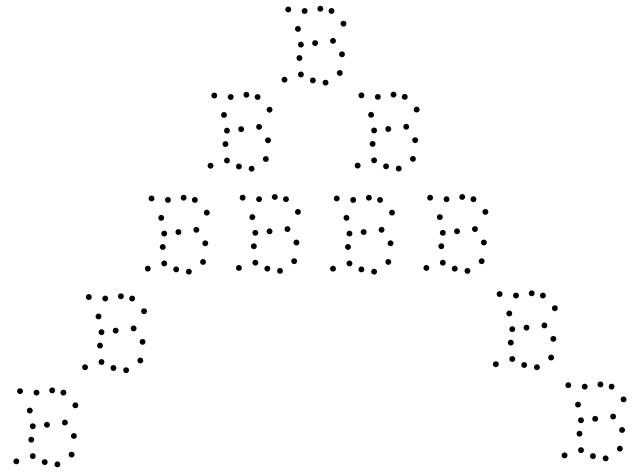
\includegraphics[width=0.5\linewidth]{./figures/exampel-dataset.png}
    \caption{}
  \end{subfigure}
  \begin{subfigure}{0.7\textwidth}
    \centering
    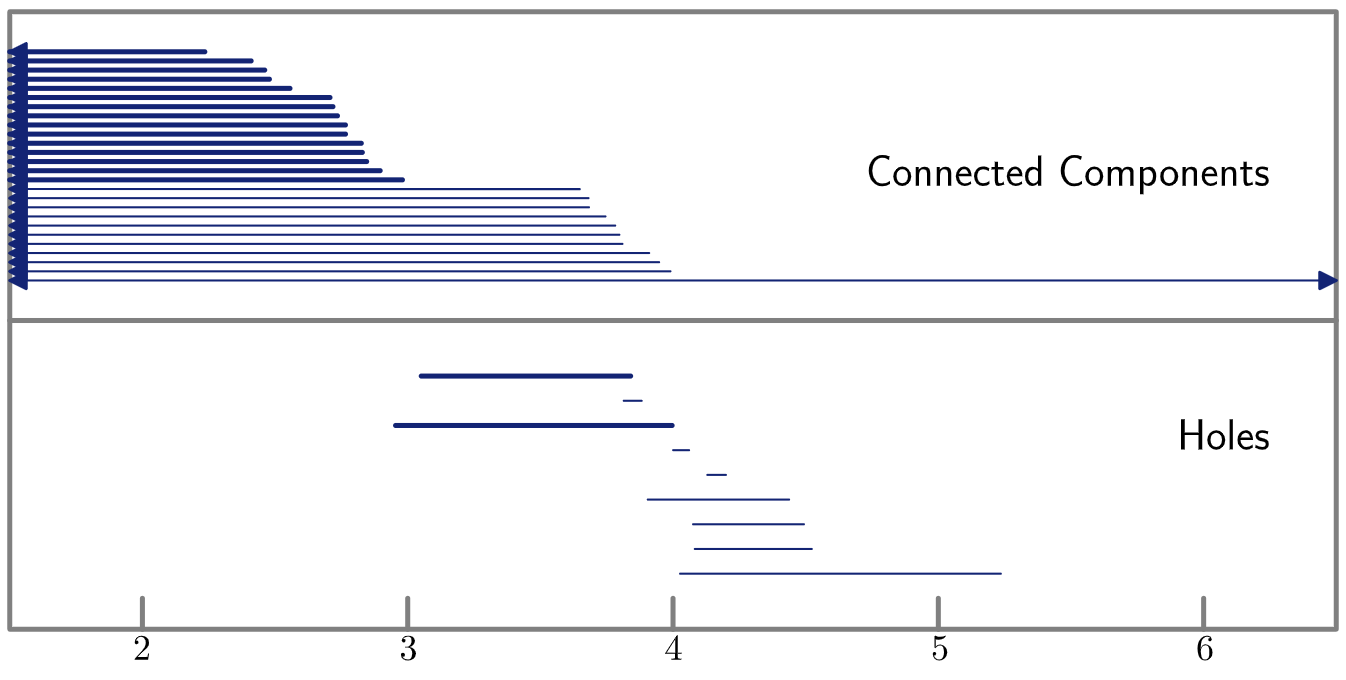
\includegraphics[width=0.7\linewidth]{./figures/example-barcode.png}
    \caption{}
  \end{subfigure}
  \caption{An example of a data set (a) and its barcode (b). The function used to produce the level sets is the distance function to our dataset. The horizontal line represents geometric scale with logarithmic graduation. Taken from \cite{oudot_2015}.}
  \label{fig:barcode-example}
\end{figure}

In general, the workflow of TDA relies on constructing a \textdef{filtration} $F(X)$ (i.e. a commutative diagram of topological spaces) which somehow encodes information about the shape of a data set $X\subset\Rb^n$, and then analyzing the structure of $F(X)$ using techniques from topology and algebraic topology \cite{botnanLesnick_2022}.
The most widely used instance of this workflow is when indexing $F(X)$ by a totally ordered set (e.g. $\Rb$ or $\Nb$).
If we wish to emphasize that a filtration is indexed by a totally ordered set, we will call it a \textdef{1-parameter filtration}.
The construction of a filtration can take many forms depending on the type of data and the kind of questions one is interested in, but a typical example is the \textdef{offset filtration}:
for each $t\in\Rb$, let $X_t=d_X^{-1}((-\infty, t])$ where $d_X\colon \Rb^n\to [0,\infty), y\mapsto\inf_{x\in X}\norm{x-y}$.
Then the offset filtration $\offset(X)$ is the collection of all $X_t$ together with the inclusion maps $s\leq t\iff X_s\hookrightarrow X_t$.
Note that $\offset$ is a functor from the poset $\Rb$ to $\Top$, the category of topological spaces.
We can then apply the $i$-th homology functor with coefficients in a field $\field$ to $\offset(X)$ to get a collection $H_i(X)$ of $\field$-vector spaces $H_i(X_t), t\in\Rb$ together with linear map induced by the inclusions.
The composition of $\offset$ and the $i$-homology gives a functor from $\Rb$ to $\Vect$, the category of $\field$-vector spaces. We will see in Chapter \ref{chap:persistenceModules} that this is an example of a (1-parameter) persistence module over $\Rb$.
There is a structure theorem \cite{BotnanCrawley_2018} that tells us that we can always decompose such a collection of vector spaces into direct sum of \textdef{interval modules}, i.e. an indicator module supported on an interval.
These, in a sense, encode the persistence of $i$-th dimensional hole in our data set across the filtration - long intervals correspond to "true" features.
The collection of all such intervals is called the \textdef{barcode} of $X$.
In Figure \ref{fig:barcode-example} we have example of a data set together with the $H_0$ and $H_1$ barcodes.
In the top barcode, the 11 lines correspond to the 11 B's which merge to form the big A around $4$, which then persists as a single cluster. 
Also note the line from 4 until a little over 5 in the bottom barcode, corresponding to the loop in the top part of the A.
For more details on algorithms used to compute barcodes, see \cite{oudot_2015,deyWang_2022}.
This process of constructing a 1-parameter filtration, applying homology to get a 1-parameter persistence module and then computing its decomposition to obtain the barcode is called \textdef{(1-parameter) persistent homology}.
\begin{figure}[h]
  \centering
  \begin{subfigure}{.45\textwidth}
    \centering
    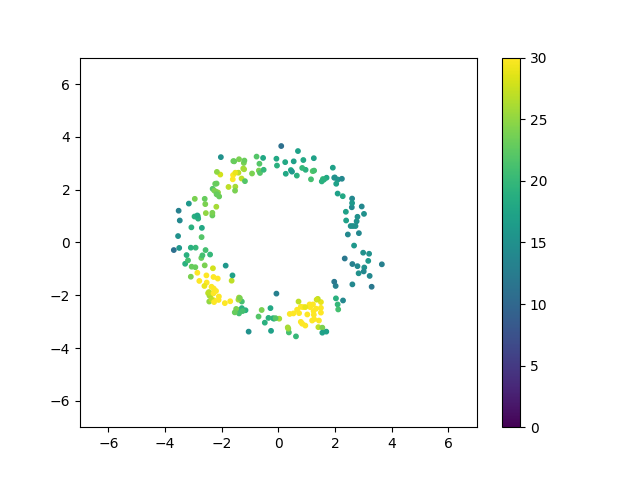
\includegraphics[width=.9\linewidth]{./figures/circle}
    \caption{}
    \label{fig:circle}
  \end{subfigure}%
  \begin{subfigure}{.45\textwidth}
    \centering
    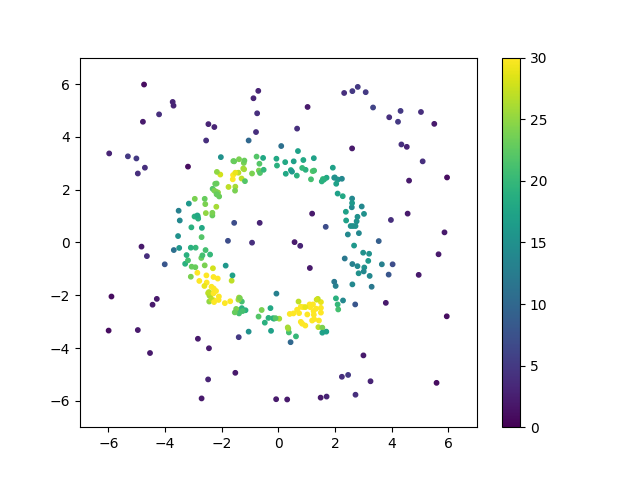
\includegraphics[width=.9\linewidth]{./figures/circle-all-points}
    \caption{}
    \label{fig:circle-all-points}
  \end{subfigure}
  \begin{subfigure}{.45\textwidth}
    \centering
    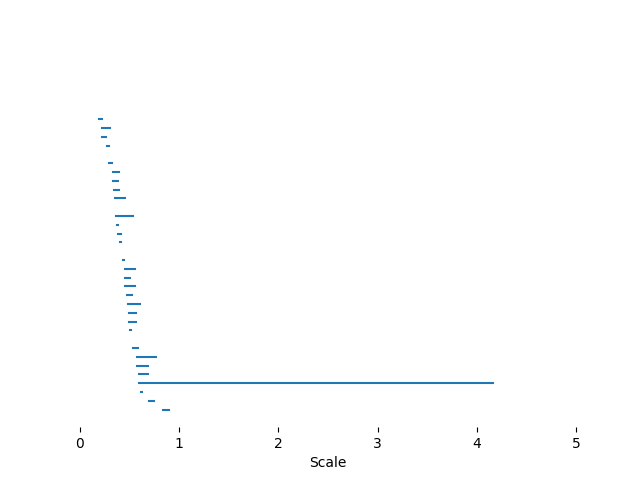
\includegraphics[width=.9\linewidth]{./figures/barcode-circle}
    \caption{}
    \label{fig:barcode-circle}
  \end{subfigure}%
  \begin{subfigure}{.45\textwidth}
    \centering
    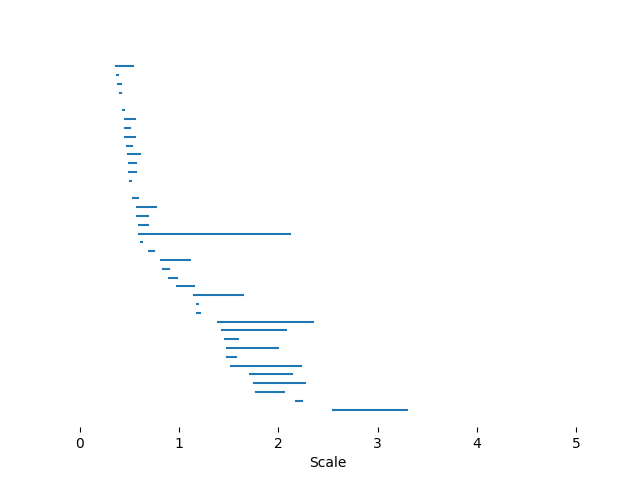
\includegraphics[width=.9\linewidth]{./figures/barcode-all-points}
    \caption{}
    \label{fig:barcode-all}
  \end{subfigure}
  \caption{
    \textbf{(a)} Circular data set colorized by local density estimate.
    \textbf{(b)} Data set from (a) with added noise.
    \textbf{(c)} The $H_1$ barcode of the data in (a).
    \textbf{(d)} The $H_1$ barcode of the data in (b).
    Taken from \cite[section 3.4]{botnanLesnick_2022}}
  \label{fig:circles-full}
\end{figure}

However, in \cite[Section 4]{BulmbergEtal_2012} it was shown that 1-parameter persistent homology is fragile.
In other words, an addition of small amount of noise can drastically change the barcode.
See for example Figure \ref{fig:circles-full}: while the $H_1$ barcode of the "clean" data set clearly captures the circular shape of the data, this is completely lost in the barcode of the noisy data.
A solution to this (and other) problems is to consider a filtration indexed by two parameters: scale (as in the offset filtration) and density threshold. This is called a \textdef{bi-filtration} or a \textdef{multi-filtration}.
A multi-filtration, instead of being a functor from a totally ordered set to $\Top$ is a functor from $P$ to $\Top$, where $P$ could be a finite product of totally ordered sets (e.g. $\Nb^2, \Rb^n$, where the partial ordering is given by $(x_i)_i\leq (y_i)_i\iff x_i\leq y_i$ for all $i$) or a different poset altogether. 
Given a multi-filtration, we can again apply homology with coefficients in a field $\field$ to obtain a multi-parameter persistence module, but unfortunately there is no decomposition similar to the barcode in the 1-parameter case \cite{gunnarAfra_2007}.
For more details regarding multi-parameter persistence and possible alternatives to the barcode see \cite{botnanLesnick_2022,botnan_2021}.
The aim of this paper is to prove the following decomposition theorem.
\begin{theorem}\label{theorem:main}
  Let $\category$ be any small category and $M\colon\category\to\Vect$ a pointwise finite dimensional (pfd) persistence module.
  Then $M$ has an essentially unique decomposition into indecomposable persistence modules.
\end{theorem}
Therefore,
\section{Outline}
In Chapter \ref{chap:persistenceModules}, we start by defining persistence modules as well as some elementary notions such as direct sum, kernels and submodules. 
We then prove that persistence modules are indeed modules over a certain algebra, and construct a tensor product.
This is followed by defining a hom functor which is right adjoint to the tensor product and proving the tensor-hom adjunction.

In Chapter \ref{chap:existence} we define the notions of pure and pure-injective modules. 
These are then used, together with the tensor-hom adjunction to prove that every pfd persistence module is pure-injective (Lemma \ref{lemma:PRepsArePure}).
This property, together with the fact that a direct summand is a pure submodule and the union of a chain of pure submodules is pure (Lemmas \ref{lemma:directSumIsPure} and \ref{lemma:unionIsPure} respectively) are the key to the proof of Lemma \ref{lemma:indecomposableSummand}, which states that every pfd persistence module has an indecomposable summand.
It is then straightforward to prove that every pfd persistence module is a direct sum of indecomposables (Theorem \ref{thm:indecomposableDecomposition}).
I would like to thank William Crawley-Boevey who shared the outline for this chapter, as well as the proof of Lemma \ref{lemma:PRepsArePure}, with Magnus Botnan which then shared them with me.

Chapter 4 starts by proving that a pfd persistence module is indecomposable if and only if it has a local endomorphism ring, which is done by a pointwise application of Fitting's Lemma, analogous to paragraphs two to five in \cite[Section 3]{BotnanCrawley_2018}.
This is then used to adapt the proof of the Krull-Remak-Schmidt-Azumaya theorem from \cite[Section 5.1]{popescu_1973}, which proves that the decomposition of a pfd persistence module into indecomposable summands is essentially unique.
\chapter{Persistence Modules}\label{chap:persistenceModules}
\section{Basic Properties}\label{sec:basicProperties}
Let $\field$ be a field and $\category$ a small category. 
Let $\Vect$ denote the category of vector fields over $\field$.
\begin{definition}
    A \textdef{persistence module} (over $\category$), or simply a \textdef{$\category$-module}, is a functor $M\colon \category\to\Vect$.
    If $\dim M_x<\infty$ for all $x\in\ob(\category)$, then we say that $M$ is pointwise finite dimensional (pfd).
    A \textdef{morphism} of persistence modules is a natural transformation between functors.
\end{definition}
Informally, given a directed graph, one can think of a persistence module as simply replacing the vertices with vector spaces and edges with linear maps in a reasonable way.
\begin{example}\label{example:persistenceModule}
    Let $\category$ be the category  \begin{tikzcd} 1 \arrow[r, "\alpha", shift left] \arrow[r, "\beta"', shift right] & 2\end{tikzcd}.
    Then a persistence module $M$ over $\category$ is given by
    \begin{center}
        \begin{tikzcd}
            \field \arrow[r, "{[1,0]^T}", shift left] \arrow[r, "{[0,1]^T}"', shift right] & \field^2
        \end{tikzcd}.
    \end{center}
    Another persistence module $M'$ is given by
    \begin{center}
        \begin{tikzcd}
            \field^2 \arrow[r, "\SmallMatrix{1}{0}{0}{1}", shift left] \arrow[r, "\SmallMatrix{0}{0}{1}{0}"', shift right] & \field^2
        \end{tikzcd}.
    \end{center}
    A morphism $\eta:M\to M'$ is given by $\eta_1=[1,0]^T\colon\field\to\field^2$ and $\eta_2=\SmallMatrix1001\colon\field^2\to\field^2$. It is straightforward to verify that
    \begin{center}
        \begin{tikzcd}
            \field \arrow[r, "{[1,0]^T}", shift left] \arrow[r, "{[0,1]^T}"', shift right] \arrow[d, "{[1,0]^T}"']         & \field \arrow[d, "\SmallMatrix{1}{0}{0}{1}"] \\
            \field^2 \arrow[r, "\SmallMatrix{1}{0}{0}{1}", shift left] \arrow[r, "\SmallMatrix{0}{0}{1}{0}"', shift right] & \field^2                                    
        \end{tikzcd}
    \end{center}
    commutes.
\end{example}
\begin{example}\label{example:intervalModule}
    If $\category$ is a totally ordered set (such as $\Nb,\Zb,\Rb$) then an \textdef{interval} $[a,b]$ is the set $\{x\in\ob(\category)\mid a\leq x\text{ and }x\leq b\}$.
    An \textdef{interval module} is a persistence module $\field^{[a,b]}:\category\to\Vect$ such that
    \[ \field^{[a,b]}_x=\begin{cases}
        \field,&x\in[a,b]\\
        0,&\text{otherwise}
    \end{cases}\qand\field^{[a,b]}_{x\to y}=\begin{cases}
        \id_{\field},&a\leq x\text{ and } y\leq b\\
        0,&\text{otherwise}
    \end{cases}. \]
\end{example}
The collection of all persistence modules over $\category$ together with natural transformations forms a functor category $\RepP$.
Since $\Vect$ is an abelian category, it follows that $\RepP$ is abelian as well \cite[p. 199]{maclane_1978}.
Explicitly, if $M, M'\in\ob(\RepP)$ then
\begin{itemize}
    \item $\Hom_{\RepP}(M,M')$ is an abelian group (and also a $\field$-vector space), and composition of morphisms is bilinear; 
    \item $\RepP$ has a zero object which is the persistence module which assigns the trivial vector space to every $x\in\ob(\category)$ and the zero map to every $\alpha\in\mor(\category)$;
    \item the \textdef{biproduct} of $M$ and $M'$ in $\RepP$, denoted by $M\oplus M'$, is the component-wise direct sum
        \[(M\oplus M')_x= M_x\oplus M'_x\qand (M\oplus M')_\alpha=M_\alpha\oplus M'_\alpha,  \]
        for $x\in\ob(\category)$ and $\alpha\in\mor(\category)$.
    \item $\RepP$ has all kernels and cokernels. For $\eta\colon M\to M'$ the \textdef{kernel}, \textdef{cokernel} and \textdef{image} of $\eta$ are the persistence modules given by $(\ker\eta)_x=\ker\eta_x, (\im\eta)_x=\im\eta_x$ and $(\coker\eta)_x=\coker\eta_x$, respectively.
    \item a morphism that is both \textdef{epi} and \textdef{monic} is an \textdef{isomorphism}.
\end{itemize}
We say that $M$ is \textdef{indecomposable} if every decomposition $M=M'\oplus M''$ implies that either $M'$ or $M''$ is trivial.
Otherwise, we say that $M$ is \textdef{decomposable}.
\begin{example}\label{example:indecomposableModule}
    Let $\category$ be the category $1\to 2$, $M'$ the $\category$-module $\field\xrightarrow{1}\field$ and $M''$ the $\category$-module $0\to\field$.
    It is easy to see that $M'$ and $M''$ are indecomposable since they are indecomposable pointwise.
    Their direct sum $M'\oplus M''$ is the $\category$-module $\field\xrightarrow{[1,0]^T}\field^2$.
\end{example}
\begin{example}
    If $\category$ is a totally ordered set, then interval modules are precisely the indecomposable persistence modules (see \cite[Section 4]{BotnanCrawley_2018} for the proof).
\end{example}
Let $M,M'\in\ob(\RepP)$. If $M'_x\subset M_x$ and $M_\alpha\vert_{M'_x}=M'_\alpha$ for all $x\in\ob(\category)$ and $\alpha\colon x\to y$ then we say that $M'$ is a \textdef{submodule} of $M$, and we write $M'\subseteq M$.
If $M'\subseteq M$ then the \textdef{quotient module} $M/M'$ is given by $(M/M')_x=M_x/M'_x$ and $(M/M')_\alpha$ is the unique map which makes the following diagram
\begin{center}
    \begin{tikzcd}
        M'_x \arrow[r, "\iota_1"] \arrow[d, "M'_\alpha"] & M_x \arrow[r, "\pi_1"] \arrow[d, "M_\alpha"] & \coker\iota_1=M_x/M'_x \arrow[d, "(M/M')_\alpha", dashed] \\
        M'_y \arrow[r, "\iota_2"]                        & M_y \arrow[r, "\pi_2"]                       & \coker\iota_2 =M_y/M'_y                                  
    \end{tikzcd}
\end{center}
commute, where $\iota_1\colon M_x'\to M_x, \iota_2\colon M_y'\to M_y$ are the inclusion maps and $\pi_1\colon M_x\to M_x/M_x', \pi_2\colon M_y'\to M_y$ are the projection maps. This map exists and is unique since $\pi_2 M_\alpha\iota_1=\pi_2\iota_2 M'_\alpha=0$ and by the universal property of the cokernel.

\section{The Tensor Product}\label{sec:theTensorProduct}
To define the tensor product $N\tensor M$ for $M\in\ob(\RepP)$ and $N\in\ob(\RepPop)$, where $\categoryop$ denotes the opposite category, we define an algebra $\pathalgebra$ and show that one can view a persistence module over $\category$ as a left module over $\pathalgebra$ (and a persistence module over $\categoryop$ as a right $\pathalgebra$-module).
We then explicitly construct the tensor product of two persistence modules.

For a morphism $\alpha\colon a\to b$ in $\category$, let $s(\alpha)=a$ be its \textdef{source} and $t(\alpha)=b$ its \textdef{tail}.
\begin{definition}
    The path algebra $\pathalgebra$ of $\category$ is the $\field$-vector space whose basis is the set of all morphisms in $\category$ and the product of two basis elements is defined by
    \[ \alpha\cdot\beta=\begin{cases}
        \alpha\circ\beta,&\text{if }t(\beta)=s(\alpha)\\
        0,&\text{otherwise}
    \end{cases}. \]
    
\end{definition}
\begin{example}\label{example:polynomialPathAlgebra}
    Let $\category$ be the category
    \begin{center}
        \begin{tikzcd}
            1 \arrow["\alpha"', loop, distance=2em, in=35, out=325]
        \end{tikzcd}.
    \end{center}
    Then the basis of $\pathalgebra$ is $\{e_1,\alpha,\alpha^2,\cdots\}$, where $e_1$ is the stationary path, and so $\pathalgebra\cong\field[t]$.
\end{example}

\begin{example}\label{example:pathAlgebra}
    Let $\category$ be the category
    \begin{center}
        \begin{tikzcd}
            1 \arrow[r, "\alpha", shift left] \arrow[r, "\beta"', shift right] & 2
        \end{tikzcd}
    \end{center}
    Then the basis of $\pathalgebra$ is $\{e_1, e_2,\alpha,\beta\}$ with multiplication table given by
    \begin{center}
        \begin{tabular}{c|cccc}
            &$e_1$&$e_2$&$\alpha$&$\beta$\\
            \hline
            $e_1$&$e_1$&0&0&0\\
            $e_2$&0&$e_2$&$\alpha$&$\beta$\\
            $\alpha$&$\alpha$&0&0&0\\
            $\beta$&$\beta$&0&0&0
        \end{tabular}
    \end{center}
    So we have an isomorphism $\pathalgebra\cong\begin{bmatrix}\field&0\\\field^2&\field\end{bmatrix}$ induced by
    \[ e_1\mapsto\begin{pmatrix}1&0\\(0,0)&0\end{pmatrix},\quad e_2\mapsto\begin{pmatrix}0&0\\(0,0)&1\end{pmatrix},\quad\alpha\mapsto\begin{pmatrix}0&0\\(1,0)&0\end{pmatrix},\quad \beta\mapsto\begin{pmatrix}0&0\\(0,1)&0\end{pmatrix}. \]
    So, for example $\alpha e_1=\alpha$ but $e_1\alpha=0$, as desired.
\end{example}
An \textdef{embedding} of categories is a functor that is fully faithful and injective on objects.
The following lemma shows that we can embed $\RepP$ inside $\Mod{\pathalgebra}{}$, the category of left $\pathalgebra$-modules, justifying the use of the word 'module' in the name of persistence module.

\begin{lemma}\label{lemma:repsAndModules}
    The map $M\mapsto\bigoplus_{x\in\ob(\category)}M_x$  defines a functor $F\colon \RepP\to\Mod{\pathalgebra}{}$.
    Moreover, $F$ is an embedding of categories.
\end{lemma}
\begin{proof}
    Let $M\in\ob(\RepP)$ and $m=\sum_{x\in\ob(\category)}m_x\in\bigoplus_{x\in\ob(\category)}M_x$ where $m_x\neq 0$ for finitely many $x\in\ob(\category)$.
    Then for $\alpha\in\mor(\category)$ define 
    \[ \alpha\cdot m\defeq M_\alpha(m_{s(\alpha)})\in M_{t(\alpha)}\subseteq \bigoplus_{x\in\ob(\category)}M_x.\]
    This gives $\bigoplus_{x\in\ob(\category)}M_x$ the structure of a left $\pathalgebra$-module.
    Let $M,M'\in\ob(\RepP)$ and $\eta\colon M\to M'$. Then
    \[ \tilde{\eta}\defeq \bigoplus_{x\in\ob(\category)}\eta_x\colon \bigoplus_{x\in\ob(\category)}M_x\to \bigoplus_{x\in\ob(\category)}M'_x \]
    is $\field$-linear. 
    We claim that it is also a $\pathalgebra$-module homomorphism, i.e. $\tilde{\eta}(\alpha m)=\alpha\tilde{\eta}(m)$ for $\alpha\in\mor(\category)$.
    Indeed, for $\alpha\colon a\to b$ we have that
    \[ \alpha\tilde{\eta}\left(\sum_{x\in\ob(\category)}m_x\right)=\alpha\sum_{x\in\ob(\category)}\eta_x(m_x)=M'_\alpha(\eta_a(m_a))\stackrel{(*)}{=}\eta_b(M_\alpha(m_a))=\tilde{\eta}(\alpha m), \]
    where $(*)$ holds since $\eta$ is a natural transformation.
    Thus, $F$ is a functor.

    The map $\eta\mapsto F(\eta)$ is injective since $F(\eta)=0$ implies $\eta=0$, and it is surjective since a $\pathalgebra$-module homomorphism $f\colon F(M)\to F(M')$ defines a natural transformation $\eta_x=f\vert_{M_x}$.
    This is well-defined since $f(e_x m)=f(e_x^2 m)=e_x f(e_x m)\in M_x$, so $f\vert_{M_x}\colon M_x\to M'_x$.
    Thus, $F$ is fully faithful.
    Moreover, if $F(M)=0$, then $M_x=0$ for all $x\in\ob(C)$ and it follows that $M=0$, so $F$ is injective on objects of $\RepP$.
\end{proof}
\begin{remark}
    The functor in Lemma \ref{lemma:repsAndModules} is in fact an equivalence of categories when $\category$ is finite (see \cite[Theorem III.1.6]{assemSkowronskiSimson_2006} for the details), but it fails to be essentially surjective when $\category$ is infinite.
\end{remark}
\begin{example}
    Let $\category$ be the category from Example \ref{example:pathAlgebra}.
    Then $\pathalgebra\cong\begin{bmatrix}
        \field&0\\
        \field^2&\field
    \end{bmatrix}$.
    Let $X$ be a left $\pathalgebra$-module and let $M$ be the $\category$ module
    \begin{tikzcd}
        e_1X \arrow[r, "\varphi_\beta"', shift right] \arrow[r, "\varphi_\alpha", shift left] & e_2X
    \end{tikzcd}
    where $\varphi_\alpha(e_1 m)=\alpha m$ and $\varphi_\beta(e_1 m)=\beta m$ for $m\in X$.
    This is well-defined since $\varphi_\alpha(m)=\alpha m=e_2\alpha m\in e_2 X$ and similarly for $\varphi_\beta$.
    Then $F(M)$ is the $\pathalgebra$-module $e_1X\oplus e_2X$ with the left action given by
    \[ \begin{pmatrix}
        a&0\\
        (b,c)& d
    \end{pmatrix}\begin{pmatrix}
        m_1\\m_2
    \end{pmatrix}=\begin{pmatrix}
        am_1\\
        b \alpha m_1+c \beta m_1+dm_2
    \end{pmatrix}. \]
    Since
    \[ \begin{pmatrix}
        1&0\\(0,0)&0
    \end{pmatrix}\begin{pmatrix}
        a&0\\(b,c)&d
    \end{pmatrix}=\begin{pmatrix}
        a&0\\0&0
    \end{pmatrix}=ae_1 \]
    and
    \[ \begin{pmatrix}
        0&0\\(0,0)&1
    \end{pmatrix}\begin{pmatrix}
        a&0\\(b,c)&d
    \end{pmatrix}=\begin{pmatrix}
        0&0\\(b,c)&d
    \end{pmatrix}=b\alpha+c\beta+de_2 \]
    it follows that $\begin{pmatrix}e_1 A m\\ e_2 A m\end{pmatrix}=A\begin{pmatrix}e_1 m\\ e_2 m\end{pmatrix}$ for $A\in\pathalgebra$ and so $X\to F(M), m\mapsto\begin{pmatrix}e_1m\\ e_2m\end{pmatrix}$ is a $\pathalgebra$-module isomorphism.
    Thus, the functor $F:\RepP\to\Mod{\pathalgebra}{}, M\to\bigoplus_{x\ob(\category)}M_x$ is essentially surjective and so an equivalence of categories.
\end{example}


Let $M\in\ob(\RepP)$ and $N\in\ob(\RepPop)$.
In light of Lemma \ref{lemma:repsAndModules}, we will slightly abuse notation, and identify a persistence module $M$ with the left $\pathalgebra$-module $\bigoplus_{x\in\ob(C)}M_x$.
Similarly, we identify $N$ with the left $\pathalgebraop$-module $\bigoplus_{x\in\ob(\category)}N_x$ (which is the same as a right $\pathalgebra$-module by defining $n\cdot\alpha\defeq\alpha^{\op}\cdot n$). 

Let $V$ be any $\field$-vector space. 
We say that a map $\varphi\colon N\times M\to V$ is \textdef{$\category$-balanced} if it is $\field$-bilinear and $\varphi(n,\alpha m)=\varphi(\alpha^{\op}n, m)$.
For fixed $M$ and $N$, the collection of all $\category$-balanced maps out of $N\times M$ forms a category $\comma{N\times M}{\Vect}$: if
\[ \varphi\colon N\times M\to V\qand \psi\colon N\times M\to W \]
are $\category$-balanced, then a morphism $\varphi\to \psi$ is a $\field$-linear map $f\colon V\to W$ which makes the following diagram
\begin{center}
    \begin{tikzcd}
        &  & V \arrow[dd, "f"] \\
        N\times M \arrow[rru, "\varphi"] \arrow[rrd, "\psi"] &  &                   \\
        &  & W                
    \end{tikzcd}
\end{center}
commute.
An initial object in this category is called a \textdef{tensor product} of $M$ and $N$.
We show that the tensor product exist by explicitly constructing one.
\begin{proposition}
    A tensor product of $M\in\ob\left(\RepP\right)$ and $N\in\ob\left(\RepPop\right)$ exists and is unique up to isomorphism.
\end{proposition}
\begin{proof}
    Let $F$ be the free vector space generated by the set $N\times M$ and $R$ be the subspace of $F$ generated by all elements of the following types
    \begin{align*}
        (n,m+m')-&(n,m)-(n, m')\\
        (n+n', m)-&(n,m)-(n',m)\\
        (cn, m)-&(n, cm)-c(m,n)\\
        \left(n,\alpha m\right)&-\left(\alpha^{\op}n, m\right)
    \end{align*}
    for $m,m'\in M$, $n,n'\in N$, $c\in\field$ and $\alpha\in\mor(\category)$.
    We have a canonical injection $\iota\colon M\times N\to F$ and a canonical projection $\pi\colon F\to F/R$.
    Taking their composition we get the map
    \[ \varphi=\pi\iota\colon N\times M\to F/R. \]
    By construction, $\varphi$ is $\category$-balanced. 
    We claim that it is a tensor product.
    
    Let $V$ be a $\field$-vector space and $\psi\colon M\times N\to V$ be $\category$-balanced.
    By the universal property of $F$ there is an induced $\field$-linear map $h\colon F\to V$ making the following diagram commute:
    \begin{center}
        \begin{tikzcd}
            &  & F \arrow[dd, "h"] \\
            N\times M \arrow[rrd, "\psi"] \arrow[rru, "\iota", hook] &  &\\
            &  & V                
        \end{tikzcd}
    \end{center}
    Since $\psi$ is $\category$-balanced, $R\subseteq\ker h$. 
    Hence, by the universal property of quotients there is linear map $g:F/R\to V$ such that the diagram
    \begin{center}
        \begin{tikzcd}
            &  & F/R \arrow[dd, "g"] \\
            F \arrow[rrd, "\psi"] \arrow[rru, "\pi", two heads] &  &                           \\
            &  & V                        
        \end{tikzcd}
    \end{center}
    commutes. 
    Since $\varphi=\pi\iota$ it follows that the diagram
    \begin{center}
        \begin{tikzcd}
            &  & F \arrow[dd, "h"] \arrow[rrd, "\pi", two heads] &  &                      \\
            N\times M \arrow[rrd, "\psi"] \arrow[rru, "\iota", hook] \arrow[rrrr, "\varphi", bend left=49, shift left=3] &  &                                               &  & F/R \arrow[lld, "g"] \\
            &  & V                                             &  &                     
        \end{tikzcd}
    \end{center}
    commutes. 
    suppose that $g'\colon F/R\to V$ is another linear map which makes the above diagram commute. 
    Then $g'\pi\iota=g'\varphi=\psi=g\pi\iota=h\iota$. 
    By uniqueness of $h$ it follows that $g'\pi=h=g\pi$ and since $\pi$ is an epimorphism, we have $g=g'$.
    Thus $g$ is unique.
    
    We conclude that $(\varphi,F/R)$ is a tensor product of $M$ and $N$. 
    Since it is an initial object in the category $\comma{N\times M}{\Vect}$, it must be unique up to isomorphism.
\end{proof}
We call $(\varphi, F/R)$ \textdef{the} tensor product of $M$ and $N$. 
The vector space $F/R$ is denoted by $N\tensor M$ and for $y\in M, x\in N$ we write $\varphi(x,y)=x\otimes y$.

Let $M_1,M_2\in\ob\left(\RepP\right)$, $N_1,N_2\in\ob\left(\RepPop\right)$, $\eta\colon M_1\to M_2$ and $\theta\colon N_1\to N_2$. 
Then the map $N_1\times M_1\to N_2\tensor M_2$ given by $(x,y)\mapsto \eta(x)\otimes \theta(y)$ is $\category$-balanced and so there is a unique linear map $\eta\otimes \theta\colon N_1\tensor M_1\to N_2\tensor M_2$ that send $x\otimes y$ to $\eta(x)\otimes \theta(y)$.
Hence, the tensor product defines a functor $\RepPop\times \RepP\to\Vect$.

\begin{example}\label{example:tensorProduct}
   Let $\category$ be the same as in Example \ref{example:pathAlgebra},
   $M$ the persistence module
   \begin{center}
        \begin{tikzcd}
            \field \arrow[r, "{[1,0]^T}", shift left] \arrow[r, "{[0,1]^T}"', shift right] & \field^2
        \end{tikzcd}
   \end{center}
   over $\category$ and $N$ the persistence module
   \begin{center}
        \begin{tikzcd}
            \field & \field \arrow[l, "1"', shift right] \arrow[l, "0", shift left]
        \end{tikzcd}
   \end{center}
   over $\categoryop$. 
   Let $\varepsilon_1$ and  $(\varepsilon_2, \varepsilon_3)$ be a basis of $M_1$ and $M_2$ respectively.
   Similarly, let $\delta_1, \delta_2$ be a basis of $N_1$ and $N_2$ respectively.
   To compute the tensor product we need to quotient $\Span\{\delta_1\otimes\varepsilon_1,\delta_2\otimes\varepsilon_2,\delta_2\otimes\varepsilon_3\}$ by the relations induced by morphisms in $\category$.
   Namely,
   \begin{align*}
    \delta_2\otimes\alpha\varepsilon_1-\alpha^{\op}\delta_2\otimes\varepsilon_1&=\delta_2\otimes\varepsilon_2-\delta_1\otimes\varepsilon_1\\
    \delta_2\otimes\beta\varepsilon_1-\beta^{\op}\delta_2\otimes\varepsilon_1&=\delta_2\otimes\varepsilon_3-0
   \end{align*}
   and so,
   \[ N\tensor M=\Span\{\delta_1\otimes\varepsilon_1,\delta_2\otimes\varepsilon_2,\delta_2\otimes\varepsilon_3\}/(\delta_2\otimes\varepsilon_2-\delta_1\otimes\varepsilon_1,\delta_2\otimes\varepsilon_3)\cong\field \]
   
   Alternatively, we can compute it using the path algebra of Example \ref{example:pathAlgebra}.
   Then $M\cong\begin{bmatrix}\field&0\\\field^2&0\end{bmatrix}=\pathalgebra\cdot e_1$ as a left $\pathalgebra$-module and so
   \[ N\tensor M\cong N\otimes_{\pathalgebra} \pathalgebra\cdot e_1=N\cdot e_1=\field. \]
\end{example}
\begin{lemma}\label{lemma:tensorRightExact}
    For $N\in\ob(\RepPop)$, the functor $N\tensor -:\RepP\to\Vect$ is right exact
\end{lemma}
\begin{proof}
    Let 
    \begin{equation}\label{eq:exactSeq}
        M\xrightarrow{\eta} M'\xrightarrow{\theta} M''\to 0
    \end{equation}
    be an exact sequence of persistence modules over $\category$. 
    We want to show that
    \begin{equation}\label{eq:tensorRightExact}
        N\tensor M\xrightarrow{\id_N\otimes\eta}N\tensor M'\xrightarrow{\id_N\otimes\theta}N\tensor M''\to 0
    \end{equation}
    is exact.
    For all $n\in N$ and $m\in M$ we have that $n\otimes(\theta\eta)(m)=0$ so $\im(\id_N\otimes\eta)\subseteq\ker(\id_N\otimes\theta)$, and we have an induced map
    \[ \phi:N\tensor M'/\im(\id_N\otimes\eta)\to N\tensor M''. \]
    To show that (\ref{eq:tensorRightExact}) is exact, it suffices to prove that $\phi$ is an isomorphism.
    We show this by constructing an inverse map.
    For every $m\in M''$, choose $m'\in M'$ such that $\theta(m')=m$ and define
    \[ N\times M''\to N\otimes M'/\im(\id_N\otimes\eta),\, (n,m)\mapsto n\otimes m'. \]
    This map is independent of the choice of $m'$, since if $m''\in M'$ is another element such that $\theta(m'')=m$ then $m''-m'\in\im\eta$ by the exactness of (\ref{eq:exactSeq}) and so
    \[ n\otimes m''-n\otimes m'=n\otimes(m''-m')\in\im(\id_N\otimes \eta). \]
    Since the map is $\category$-balanced it induces a map $\psi:N\tensor M''\to N\tensor M'/\im(\id_N\otimes \eta)$.
    Then $(\psi\phi)(n\otimes m)=\psi(n\otimes\theta(m))=n\otimes m$ and $(\phi\psi)(n\otimes m)=\phi(n\otimes m')=n\otimes m$ and so $\phi$ is an isomorphism.
\end{proof}

\section{Duality}\label{sec:duality}
Pointwise duality with the field $\field$ of a persistence module $M\colon \category\to\Vect$ gives a persistence module $DM\colon\categoryop\to\Vect$.
In this section we show that duality is a contravariant exact functor and satisfies $D^2M\cong M$ if $M$ is a pfd.
If $U,V$ are $\field$-vector spaces and $T\colon U\to V$ then we denote $\Hom_{\field}(V,\field)$ by $V^*$ and the map $U^*\to V^*, f\mapsto f\circ T$ by $T^*$.
\begin{lemma}\label{lemma:dualityIsExact}
    Pointwise duality defines a contravariant exact functor $D\colon\RepP\to\RepPop$
\end{lemma}
\begin{proof}
    Dualizing each vector space and linear map in $M$ we get
    \[ (DM)_x={M_x}^*\quad(DM)_{\alpha^{\op}}={M_\alpha}^*\colon M_y^*\to M_x^*, f\mapsto f\circ M_\alpha \]
    for all $x,y\in\ob(\category)$ and $\alpha\colon x\to y$. 
    If $\eta\colon M\to M'$ is a morphism of persistence modules then $D\eta\colon DM'\to DM$ is given by $(D\eta)_x(f)=f\circ \eta_x$ for $x\in\ob(\category)$ and $f\in (M_x')^*$.
    It is immediate that $D\id_M=\id_{DM}$ and $D(\eta\theta)=(D\theta)(D\eta)$, so $D$ is a contravariant functor.

    Let $0\to M^1\xrightarrow{\eta} M^2\xrightarrow{\theta} M^3\to $ be an exact sequence of persistence modules. 
    Since $\field$ is an injective $\field$-module, it follows that $\Hom_{\field}(-, \field)\colon \Vect\to\Vect$ is exact and so
    \[ 0\to DM^3_x\xrightarrow{\theta_x^*} DM^2_x\xrightarrow{\eta_x^*}DM^1_x\to 0 \]
    is exact for all $x\in\ob(\category)$. 
    Hence, $(\ker D\theta)_x=\ker (D\theta)_x=\ker\theta_x^*=0$, $(\im D\eta)_x=\im\eta_x^*=DM^1_x$ and $(\ker D\eta)_x=\ker\eta_x^*=\im\theta_x^*=(\im D\theta)_x$ for all $x$, so $0\to DM_3\xrightarrow{D\theta} DM_2\xrightarrow{D\eta} DM_1\to 0$ is exact.
\end{proof}


Note that $DM=\bigoplus_{x\in\ob(\category)}\Hom_{\field}(M_x,\field)$ and so for $f=\sum_{x\in\ob(\category)}f_x\in DM$ we have that $(\alpha^{\op}f)_x=M_\alpha^*(f_{s(\alpha^{op})})=f_{t(\alpha)}\circ M_\alpha$ if $x=t(\alpha)$ and 0 otherwise.
In other words, for $m\in M$ and $f\in DM$ we have
\[ f(\alpha m)=f_{t(\alpha)}(M_\alpha(m_{s(\alpha)}))=(\alpha^{op}f)(m), \]
which better emphasizes the $\pathalgebraop$-module structure of $DM$.

We also denote the pointwise duality functor $\RepPop\to\RepP$ by $D$.

\begin{lemma}\label{lemma:doubleDual}
    Let $M\in\ob(\RepP)$ be pfd. Then $D^2M\cong M$.
\end{lemma}
\begin{proof}
    Since $M_x$ is finite dimensional for all $x\in\ob(\category)$, we have the canonical isomorphism $\phi_x\colon M_x\to\left( D^2M \right)_x$
    given by $\phi_x(m)(f)=f(m)$ for $m\in M_x$ and $f\in (DM)_x$.
    
    If $\alpha\colon x\to y$ is a morphism in $\category$, $m\in M_x$ and $f\colon M_y\to\field$ then
    \begin{align*}
        \left( (D^2M)_\alpha\circ\phi_x \right)(m)(f)&=\left(\phi_x(m)\circ (DM)_{\alpha^{\op}}  \right)(f)\\
        &=\phi_x(m)\left( f\circ M_\alpha \right)\\
        &=(f\circ M_\alpha)(m)\\
        &=\left( \phi_y\circ M_\alpha \right)(m)(f)
    \end{align*}
    so the following diagram commutes
    \begin{center}
        \begin{tikzcd}
            M_x \arrow[d, "\phi_x"] \arrow[r, "M_\alpha"] & M_y \arrow[d, "\phi_y"] \\
            (D^2M)_x \arrow[r, "(D^2M)_\alpha"]           & (D^2M)_y               
        \end{tikzcd}.
    \end{center}
    Thus, $\phi$ is a natural isomorphism.
\end{proof}
\begin{remark}
    The fact that $\phi$ in the above proof is a natural isomorphism, is equivalent to it being a $\pathalgebra$-module isomorphism. 
    Thus, the naturality condition is equivalent to $\phi(\alpha m)=\alpha\phi(m)$ which follows from
    \[\phi(\alpha m)(f)=f(\alpha m)=(\alpha^{\op}f)(m)=\phi(m)(\alpha^{\op}f)=(\alpha\phi(m))(f).\]
\end{remark}

\section{Tensor-Hom Adjunction}\label{sec:tensorHomAdjunction}
Let $N\in\ob(\RepPop)$.
We saw in Section \ref{sec:theTensorProduct} that the tensor product defines a functor $N\tensor -\colon \RepP\to\Vect$.
In this section we show that the tensor product has a right adjoint functor and construct it explicitly.

For a right $\pathalgebra$-module $X$, we can take its dual as a $\field$-vector space to get the left $\pathalgebra$-module $X^*=\Hom_{\field}(X,\field)$ endowed with the right $\pathalgebra$-module structure given by $\alpha\varphi(a)=\varphi(\alpha^{\op} a)$ for $\alpha\in\mor(\category),\varphi\in X^*$ and $m\in X$.
For a $\categoryop$-module $N$, pointwise duality gives a $\pathalgebra$-module 
\[ DN=\bigoplus_{x\in\ob(\category)}\Hom_{\field}(N_x,\field)\subseteq\prod_{x\in\ob(\category)}\Hom_{\field}(N_x,\field)=\Hom_{\field}(N,\field). \]
Thus, it is natural to generalize duality to a functor $\hom_{\field}(N, -)\colon\Vect\to\RepP$ given by
\[ \hom_{\field}(N, V)=\bigoplus_{x\in\ob(\category)}\Hom_{\field}(N_x,V)\subseteq\Hom_{\field}(N, V),\]
where $V$ is a $\field$-vector space.
Explicitly, $\hom_{\field}(N, V)$ is the $\category$-module given by $(\hom_{\field}(N, V))_x=\Hom_{\field}(N_x,V)$ and $(\hom_{\field}(N, V))_\alpha=N_{\alpha^{\op}}^*$ and for a $\field$-linear map $f:V\to W$, $(\hom_{\field}(N, f))_x=f\circ -$.
In particular, we have that $\hom_{\field}(N,\field)=DN$.
\begin{proposition}\label{prop:TensorHomAdjunction}
    Let $N\in\ob(\RepPop)$. 
    Then $\hom_{\field}(N, -)$ and $N\tensor -$ are adjoint functors.
\end{proposition}
\begin{proof}
    Let $M\in\ob(\RepP)$ and $V$ a $\field$-vector space.
    Define 
    \[\phi_{M,V}\colon\Hom_{\field}(N\tensor M, V)\to\Hom_{\RepP}(M,\hom_{\field}(N, V))\]
    by $\phi_{M,V}(f)(m)(n)=f(n\otimes n)$.
    Then
    \[ \phi(f)(\alpha m)(n)=f(n\otimes\alpha m)=f(\alpha^{\op} n\otimes m)=\phi(f)(m)(\alpha^{\op}n)=(\alpha\phi(f)(m))(n), \]
    where the last equality follows since $\phi(f)(m)\in\hom_{\field}(N,V)\subseteq\Hom_{\field}(N,V)$ and by definition of the module structure of $\Hom_{\field}(N, V)$.
    Thus, $\phi(f)$ is a morphism of $\category$-modules, and it follows that $\phi$ is well-defined.
    
    To show that $\phi_{M,V}$ is an isomorphism, we construct an inverse map.
    Let $\eta:M\to\hom_{\field}(N,V)$ be a natural transformation. 
    The map $N\times M\to V, (n,m)\mapsto \eta(m)(n)$ is $\category$ balanced, and so there exists a unique $\bar{\eta}:N\tensor M\to V$ such that $\bar{\eta}(n\otimes m)=\eta(m)(n)$.
    Let $\psi_{M,V}:\Hom_{\RepP}(M,\hom_{\field}(N,V))\to\Hom_{\field}(N\tensor M, V), \eta\mapsto\bar{\eta}$.
    Since
    \[ (\psi_{M,V}\phi_{M,V})(f)(n\otimes m)=\psi_{M, V}(\phi_{M,V}(f))(n\otimes m)=\phi_{M,V}(f)(m)(n)=f(n\otimes m) \]
    and
    \[ (\phi_{M, V}\psi_{M,V})(\eta)(m)(n)=\phi_{M,V}(\bar{\eta})(m)(n)=\bar{\eta}(n\otimes m)=\eta(m)(n), \]
    it follows that $\psi_{M,V}=\phi_{M,V}^{-1}$ and so $\phi_{M,V}$ is an isomorphism.
    
    To show this isomorphism is natural, let $M',M''\in\ob(\RepP)$, $\eta\colon M'\to M''$, $V_1,V_2\in\ob(\Vect)$ and $g:V_1\to V_2$.
    Then
    \begin{center}
        \begin{tikzcd}
            {\Hom_{\field}(N\tensor M',V_1)} \arrow[r, "{\phi_{M',V_1}}"]                                       & {\Hom_{\RepP}(M',\hom_{\field}(N, V_1))}             \\
            {\Hom_{\field}(N\tensor M'',V_1)} \arrow[u, "-\circ(\id_N\otimes\eta)"] \arrow[r, "{\phi_{M'',V_1}}"] & {\Hom_{\RepP}(M'',\hom_{\field}(N, V_1))} \arrow[u, "-\circ \eta"']
        \end{tikzcd}
    \end{center}
    commutes since
    \begin{align*}
        \phi_{M', V_1}(f\circ(\id_N\otimes\eta))(m)(n)&=f\left((\id_N\otimes\eta)(n\otimes m)\right)\\
        &=f(n\otimes\eta(m))\\
        &=\phi_{M'', V_1}(f)(\eta(m))(n)\\
        &=(\phi_{M'', V_1}(f)\circ\eta)(m)(n).
    \end{align*}
    Similarly, since
    \begin{align*}
        (\hom_{\field}(N,g)\circ\phi_{M', V_1}(f))(m)(n)&=(g\circ\phi_{M', V_1}(f))(m)(n)\\
        &=g(f(n\otimes m))\\
        &=(\phi_{M', V_2}(g\circ f))(m)(n)
    \end{align*}
    we have that
    \begin{center}
        \begin{tikzcd}
            {\Hom_{\field}(N\tensor M',V_1)} \arrow[r, "{\phi_{M',V_1}}"] \arrow[d, "g\circ -"'] & {\Hom_{\RepP}(M',\hom_{\field}(N, V_1))} \arrow[d, "{\hom_{\field}(N,g)\circ -}"] \\
            {\Hom_{\field}(N\tensor M',V_2)} \arrow[r, "{\phi_{M',V_2}}"]                        & {\Hom_{\RepP}(M',\hom_{\field}(N, V_2))}                                         
        \end{tikzcd}
    \end{center}
    commutes.
\end{proof}
The following corollary is the result we need for Chapter \ref{chap:existence}, and so we state here it for reference. 
The proof is obtained by simply taking $V=\field$ and applying the tensor-hom adjunction.
\begin{corollary}\label{cor:tensorHomAdjunction}
    Let $M\in\ob(\RepP)$ and $N\in\ob(\RepPop)$. Then
    \[ \Hom_{\field}(N\tensor M,\field)\cong\Hom_{\RepP}(M, DN) \]
    as $\field$-vector spaces. Moreover, the isomorphism is natural in $M$.
\end{corollary}
\begin{example}\label{example:tensorHomAdjunction}
    Let $\category, M$ and $N$ be as in Example \ref{example:tensorProduct}.
    A morphism $\eta\colon M\to DN$ consists of $\field$-linear maps $\eta_1\colon\field\to\field$ and $\eta_2:\field^2\to\field$ so that
    \begin{center}
        \begin{tikzcd}
            \field \arrow[d, "\eta_1"] \arrow[r, "{[1,0]^T}"] & \field^2 \arrow[d, "\eta_2"] & \field \arrow[d, "\eta_1"] \arrow[r, "{[0,1]^T}"] & \field^2 \arrow[d, "\eta_2"] \\
            \field \arrow[r, "1"]                             & \field                       & \field \arrow[r, "0"]                             & \field                      
        \end{tikzcd}
    \end{center}
    commutes. 
    In other words, $\eta_1(c)=\eta_2(c,0)$ and $0=\eta_2(0,c)$ for all $c\in\field$.
    Thus, choosing $\eta_1\in\End_{\field}(\field)\cong\field$ determines $\eta$, and it follows that $\Hom_{\RepP}(M, DN)\cong\field$.
    From Example \ref{example:tensorProduct} we know that $N\tensor M\cong\field$ and so $\Hom_{\field}(N\tensor M,\field)\cong\Hom_{\field}(\field,\field)\cong\field$.
\end{example}

\chapter{Existence of Decomposition}\label{chap:existence}
\begin{definition}
    A short exact sequence of persistence modules $0\to M\to M'\to M''\to 0$ is called \textdef{pure-exact} if $0\to N\tensor M\to N\tensor M'\to N\tensor M''\to 0$ is exact for every $N\in\ob(\RepPop)$.
    A submodule $M'\subseteq M$ is \textdef{pure} if the canonical exact sequence
    \[ 0\to M'\to M\to M/M'\to 0 \]
    is pure-exact.
\end{definition}
Note that since the tensor product is right exact (Lemma \ref{lemma:tensorRightExact}), to verify that an exact sequence of $\category$-modules $0\to M\xrightarrow{\eta} M'\to M''\to 0$ is pure, it suffices to check that $\id_N\otimes\eta$ is injective for all $\categoryop$-modules $N$.
\begin{example}\label{example:pureSubmodule}
    Let $\category$ be the category $1\to 2$, $M$ the persistence module $\field\xrightarrow{[1,0]^T}\field^2$ and $M'$ the persistence module $0\to\field$.
    We claim that $M'$ is pure in $M$.
    Let $\eta\colon M'\to M$ be given by $\eta_1=0$ and $\eta_2=[0,1]^T$, and $\theta\colon M\to M'$ be given by $\theta_1=0$ and $\theta_2=[0,1]$.
    Since $\eta$ is the inclusion map, we have a canonical exact sequence
    \[ 0\to M'\xrightarrow{\eta} M\to M/M'\to 0. \]
    Since $\theta\eta=\id_{M'}$ and for all $N\in\ob(\RepPop)$ we have that
    \[ n\otimes m=\id_{N\tensor M}(n\otimes m)=(\id_N\otimes\theta\eta)(n\otimes m)=(\id_N\otimes\theta)(\id_N\otimes\eta)(n\otimes m), \]
    it follows that $\ker(\id_N\otimes\eta)=0$.
    Thus, $\id_N\otimes\eta$ is injective and so $M'$ is pure in $M$.
\end{example}
In Example \ref{example:pureSubmodule} we have that $M=M''\oplus M'$ where $M''$ is the persistence module $\field\xrightarrow{1}\field$,
suggesting that a direct summand is a pure submodule. 
This is proven in the following lemma.
\begin{lemma}\label{lemma:directSumIsPure}
    A direct summand is a pure submodule.
\end{lemma}
\begin{proof}
    Let $M,M'\in\ob(\RepP)$. Consider the exact sequence
    \begin{equation}\label{eq:directSumExactSequence}
        0\to M\xrightarrow{\iota} M\oplus M'\to M'\to 0
    \end{equation}
    and let $N\in\ob(\RepPop)$.
    Let $\pi\colon M\oplus M'\to M$ be the projection map, so that $\pi\iota=\id_M$, and take $n\otimes m\in N\tensor M$ such that $(\id_N\otimes\iota)(n\otimes m)=n\otimes\iota(m)=0$.
    Functoriality of the tensor product gives
    \[n\otimes m=\id_{N\tensor M}(n\otimes m)=(\id_N\otimes\pi\iota)(n\otimes m)=(\id_N\otimes\pi)(n\otimes \iota(m))=0, \]
    and it follows that $\id_N\otimes\iota$ is injective.
\end{proof}

\begin{lemma}\label{lemma:unionIsPure}
    A union of a chain of pure submodules is pure.
\end{lemma}
\begin{proof}
    Let $M\in\ob(\RepP)$ and $M^1\subseteq M^2\subseteq M^3\subseteq\cdots$ a chain of pure submodules.
    We want to show that the canonical exact sequence
    \begin{equation}\label{eq:limitOfChain}
        0\to A\xrightarrow{\iota} M\xrightarrow{\pi} M/A\to 0 
    \end{equation}
    is pure-exact, where $A=\bigcup_{i=1}^\infty M^i$.
    Let $N\in\ob(\RepPop)$ and take $n\otimes m\in N\tensor A$ such that $(\id_N\otimes\iota)(n\otimes m)=0$.
    Then $m\in M^i$ for some $i\in\Nb$ and since
    \[ 0\to M^i\xrightarrow{\iota_i} M\xrightarrow{\pi_i} M/M^i\to 0 \]
    is pure-exact, it follows that $\id_N\otimes\iota_i$ is injective. Since
    \[ (\id_N\otimes\iota_i)(n\otimes m)=(\id_N\otimes\iota)(n\otimes m)=0 \]
    it follows that $n\otimes m=0$ and so $\id_N\otimes\iota$ is injective and the result follows.
\end{proof}

\begin{definition}
    A persistence module $M$ is called \textdef{injective} if the functor $\Hom_{\RepP}(-, M):\RepP\to\Vect$ is exact.
    It is \textdef{pure-injective} if $\Hom_{\RepP}$ is exact on pure-exact sequences.
\end{definition}

\begin{lemma}\label{lemma:PRepsArePure}
    A pfd persistence module is pure-injective.
\end{lemma}
The following proof is due to William Crawley-Boevey \cite{crawley-boevey_2017}.
\begin{proof}
    Let $M\in\ob(\RepP)$ be pfd and $0\to M^1\to M^2\to M^3\to 0$ be a pure-exact sequence of persistence modules.
    Then
    \[0\to DM\tensor M^1\to DM\tensor M^2\to DM\tensor M^3\to 0\] 
    is exact, and we can dualize to get that
    \[ 0\to (DM\tensor M_3)^*\to (DM\tensor M_2)^*\to (DM\tensor M_1)^*\to 0 \]
    is exact.
    By Corollary \ref{cor:tensorHomAdjunction} and Lemma \ref{lemma:doubleDual} it follows that 
    \[ (DM\tensor M^i)^*\cong\Hom_{\RepP}(M^i, D^2M)\cong\Hom_{\RepP}(M^i, M),\quad i=1,2,3.\]
    Since this isomorphism is natural, we conclude that
    \[ 0\to\Hom_{\RepP}(M^3, M)\to \Hom_{\RepP}(M^2,M)\to \Hom_{\RepP}(M^1, M)\to 0 \]
    is exact, showing that $M$ is pure-injective. 
\end{proof}

\begin{lemma}\label{lemma:pureIsDirectSum}
    If $M$ is a pure-injective persistence module, then every pure-exact sequence $0\to M\xrightarrow{\eta} M'\xrightarrow{\theta} M''\to 0$ splits.
\end{lemma}
\begin{proof}
    Since $M$ is pure-injective we have that
    \[ 0\to \Hom_{\RepP}(M'', M)\to \Hom_{\RepP}(M',M)\to \Hom_{\RepP}(M,M)\to 0 \]
    is exact. In particular there is $\zeta\in\Hom_{\RepP}(M',M)$ such that $\zeta\eta=\text{id}_M$.
    Consider the map $\varphi:M'\to M\oplus M''$ given by $\varphi(x)=(\zeta(x),\theta(x))$.
    Then the diagram
    \begin{center}
        \begin{tikzcd}
            0 \arrow[r] & M \arrow[r, "\eta"] \arrow[d, "\text{id}_M"] & M' \arrow[r, "\theta"] \arrow[d, "\varphi"] & M'' \arrow[r] \arrow[d, "\text{id}_{M''}"] & 0 \\
            0 \arrow[r] & M \arrow[r, "\iota"]                      & M\oplus M'' \arrow[r, "\pi"]            & M'' \arrow[r]                              & 0
            \end{tikzcd}
    \end{center}
    commutes.
    Since $\RepP$ is an abelian category we can use the Five Lemma to conclude that $\varphi$ is an isomorphism.
\end{proof}

The following two proofs are analogous to paragraphs three and four (respectively) in \cite[p. 163]{jensen_lenzing_1989}
\begin{lemma}\label{lemma:indecomposableSummand}
    If $M$ is a nonzero pfd persistence module, then it has an indecomposable summand.
\end{lemma}
\begin{proof}
    Let $m\in M$ and 
    \[S=\{N\subseteq M\mid N\text{ is pure in }M\text{ and }m\not\in N\}.\]

    The union $N$ of any chain $N_1\subseteq N_2\subseteq\cdots$ in $S$ is again pure by Lemma \ref{lemma:unionIsPure} and $m\not\in N$. 
    Thus, $N\in S$.
    By Zorn's lemma it follows that there is a maximal element $N\in S$.
    Now, $N$ is pure in $M$ so the sequence $0\to N\to M\to M/N\to 0$ is pure-exact and $N$ is pfd so it is pure-injective by Lemma \ref{lemma:PRepsArePure}.
    Thus, it follows by Lemma \ref{lemma:pureIsDirectSum} that $M\cong N\oplus M/N$. 
    Note that $M/N$ is non-zero since $m\in M/N$.
    Suppose that $M/N$ decomposes as $U\oplus U'$.
    Then $N\oplus U$ and $N\oplus U'$ are direct summands of $M$, so pure in $M$ by Lemma \ref{lemma:directSumIsPure} and since they can't both contain $m$, one of them contradicts the maximality of $N$.
\end{proof}

\begin{theorem}\label{thm:indecomposableDecomposition}
    If $M$ is a nonzero pfd persistence module, then it is a direct sum of indecomposables.
\end{theorem}
\begin{proof}
    Let $S=\{N\subset M\mid N\text{ is indecomposable}\}$, which is non-empty by the previous lemma, and 
    \[\Uc=\{I\subset S\mid\bigoplus_{N\in I}N\text{ is direct and pure in }M\},\]
    which is non-empty by the previous lemma and Lemma \ref{lemma:directSumIsPure}.
    Again by Zorn's lemma it follows that $\Uc$ has a maximal element $I$ and $M'=\bigoplus_{N\in I} N$ is direct and pure in $M$.
    Then $M=M'\oplus M''$ where $M''$ must be zero, otherwise it would have an indecomposable summand, contradicting the maximality of $I$.
    Thus $M=\oplus_{N\in I}N$. 
\end{proof}
\chapter{Uniqueness of Decomposition}\label{chap:uniqueness}
The following lemma, as well as Lemma \ref{lemma:indecpomposableIffLocal}, were adapted from \cite[Section 3]{BotnanCrawley_2018}.
\begin{lemma}
    Let $M$ be a pfd persistence module. 
    Then every endomorphism $\eta\colon M\to M$ induces a decomposition $M=M'\oplus M''$, where $M'_x=\im\eta_x^{n_x}$ and $M''_x=\ker\eta_x^{n_x}$ for some $n_x\in\Nb$. 
\end{lemma}
\begin{proof}
    Suppose $M$ is indecomposable and let $\eta\in\End_{\RepP}(M)$. 
    Then we have a linear endomorphism $\eta_x\colon M_x\to M_x$ for each $x\in\ob(\category)$.
    Since $M_x$ is a finite dimensional vector space, the Fitting lemma gives us a decomposition
    \[ M_x=\im(\eta^n_x)\oplus\ker(\eta^n_x) \]
    for $n$ sufficiently large.

    Let $\alpha\colon x\to y$ be a morphism in $\category$. Then $M_\alpha\eta_x=\eta_yM_\alpha$ since $\eta\colon M\to M$ is a natural transformation.
    Furthermore, taking $n$ sufficiently large for the decomposition of $M_x$ and $M_y$ we have $M_\alpha\eta^n_x=\eta^n_yM_\alpha$ so $M_\alpha\left(\im(\eta_x^n)\right)\subseteq\im(\eta_y^n)$ and $M_\alpha\left(\ker(\eta^n_x)\right)\subseteq\ker(\eta^n_y)$.
    Thus, the decomposition $\im(\eta^n_x)\oplus\ker(\eta^n_x)$ for each $x$ gives a decomposition $M=M'\oplus M''$ as persistence modules, where $M'_x=\im(\eta_x^{n_x})$ and $M''_x=\ker(\eta_x^{n_x})$ for $n_x\in\Nb$ sufficiently large.
\end{proof}
\begin{corollary}\label{cor:ImKerDecomposition}
    Let $M$ be a pfd persistence module and $\eta\colon M\to M$ an idempotent endomorphism.
    Then $M=\im\eta\oplus\ker\eta$.
\end{corollary}
\begin{proof}
    We have that $M'_x=\im\eta_x^{n_x}=\im\eta_x$ and $M''_x=\ker\eta_x^{n_x}=\ker\eta_x$ for all $x\in\ob(\category)$ and the result follows.
\end{proof}


\begin{lemma}\label{lemma:indecpomposableIffLocal}
    Let $M$ be a pfd persistence module. 
    Then $M$ is indecomposable if and only if $\End_{\RepP}(M)$ is local.
\end{lemma}
\begin{proof}
    Suppose $M$ is indecomposable.
    Let $\eta\in\End_{\RepP}(M)$ and let $M=M'\oplus M''$ be the corresponding decomposition.
    Since $M$ is indecomposable, we have $M=M'$ or $M=M''$.
    If $M=M'$, then $\im\eta_x^{n_x}=M_x$ and since $\im\eta_x^{n_x}\subseteq\im\eta_x$ it follows that $\im\eta_x=M_x$ for all $x\in\ob(\category)$.
    Since $\eta_x$ is a surjective endomorphism of finite dimensional vector spaces, it is an isomorphism\footnote{
        This follows from $0\to\ker\eta_x\to M_x\xrightarrow{\eta_x} M_x\to 0$ being a short exact sequence of vector spaces, so it splits, and comparing dimensions we can conclude that $\ker\eta_x=0$.
    } for all $x$ and so $\eta$ is an isomorphism. 
    Otherwise, if $M=M''$ then $\eta_x^{n_x}=0$ for all $x$ and it follows that
    \[1=1-\eta_x^{n_x}=(1-\eta_x)\left(1+\eta_x+\cdots+\eta_x^{n_x-1}\right),\]
    so $1-\eta_x$ is invertible for all $x$.
    Thus, $1-\eta$ is invertible, and it follows that $\End_{\RepP}(M)$ is local.
    
    To prove the converse, suppose $M$ is decomposable. Then $M=M'\oplus M''$ for $M',M''$ nontrivial.
    Let $\eta_x\colon M_x\to M_x$ be the projector to $M_x'$ for every $x$. It is clear that $\eta\in\End_{\RepP}(M)$ and that neither $\eta, 1-\eta$ are isomorphism.
    Thus, $\End_{\RepP}(M)$ is not local.
\end{proof}

The following lemma is analogous to \cite[Lemma 2.6]{facchini_1998}.
\begin{lemma}\label{lemma:projectionIsIso}
    Let $M',M''$ be persistence modules, $M=M'\oplus M''$ and $N\subseteq M$.
    Then $M=M'\oplus N$ if and only if $\pi_{M''}\vert_{N}\colon N\to M''$ is an isomorphism, where $\pi_{M''}$ is the canonical projection.
    If one of these conditions hold, then the canonical projection $\pi_{N}\colon M\to N$ is given by $\pi_{N}=(\pi_{M''}\vert_{N})^{-1}\pi_{M''}$.
\end{lemma}
\begin{proof}
    The map $\pi_{M''}\vert_{N}$ is injective if and only if $N\cap M'=0$ and surjective if and only if for every $m_2\in M''$ there is $m'\in N$ such that $m'=m_1+m_2$ for some $m_1\in M'$, which is the case if and only if $M''\subset N+M'$. 
    Hence, $\pi_{M''}\vert_{N}$ is bijective if and only if $M'\oplus M''=M'\oplus N$, which proves the first part.
    Suppose $M=M'\oplus M''=M'\oplus N$. 
    Let $m\in M$. 
    Then $m=\pi_{M'}(m)+\pi_{N}(m)$ so $\pi_{M''}(m)=(\pi_{M''}\pi_{M'})(m)+(\pi_{M''}\vert_{N}\pi_{N})(m)=(\pi_{M''}\vert_{N}\pi_{N})(m)$ and it follows that $\pi_{N}(m)=\left((\pi_{M''}\vert_{N})^{-1}\pi_{M''}\right)(m)$.
\end{proof}

If we have a persistence module $M=\bigoplus_{i\in I}M^i$, then for $I'\subseteq I$  let $M(I')=\bigoplus_{i\in I'}M^i$.

The following three proofs were inspired by Lemma 1.1, Lemma 1.2 and Theorem 1.3 in Chapter 5 of \cite{popescu_1973}, respectively.
\begin{lemma}\label{lemma:extractingIndecomposables}
    Let $M=\bigoplus_{i\in I} M^i$ be a pfd persistence module where $M^i$ are indecomposable.
    Let $\eta,\theta\in\End(M)$ such that $\eta+\theta=1_M$. 
    Then for any $\{i_1,i_2,\dots, i_s\}\subseteq I$ there exist submodules $N^1, N^2,\dots N^s$ such that
    \begin{enumerate}
        \item For each $k=1,\dots,s$ either $\eta$ or $\theta$ induces an isomorphism of $N^k$ with $M^{i_k}$.
        \item $M=N^1\oplus\cdots\oplus N^s\oplus M(I\setminus\{i_1,\cdots i_s\})$ 
    \end{enumerate} 
\end{lemma}
\begin{proof}
    Let $\iota_i\colon M^i\to M$ be the inclusion maps and $\pi_i\colon M\to M^i$ the associated projection maps.
    Then
    \[ \pi_i=\pi_i(\eta+\theta)=\pi_i\eta+\pi_i\theta \]
    and so
    \[ 1_{M^i}=\pi_i\iota_i=\pi_i \eta\iota_i+\pi_i \theta\iota_i. \]
    Since $\End(M^i)$ is local for each $i\in I$ (by Lemma \ref{lemma:indecpomposableIffLocal}), it follows that one of $\pi_i\eta\iota_i$ and $\pi_i\theta\iota_i$ is an isomorphism.
    Suppose that $\pi_{i_1} \eta\iota_{i_1}$ is an isomorphism and let $N^1=\im \eta\iota_{i_1}$.
    Since $\pi_{i_1} \eta\iota_{i_1}$ is an isomorphism, it follows that $\pi_{i_1}\vert_{N^1}\colon N^1\to M^{i_1}$ is an isomorphism and so by Lemma \ref{lemma:projectionIsIso} it follows that $M=N^1\oplus M(I\setminus\{i_1\})$.
    Repeating the argument for $s$ times we obtain $N^1,N^2,\dots, N^s$ with the desired properties.
\end{proof}


\begin{lemma}\label{lemma:idempotentInduceIso}
    Let $M=\bigoplus_{i\in I}M^i$ be a pfd persistence module with $M^i$ indecomposable.
    If $\eta\colon M\to M$ is nonzero and $\eta^2=\eta$ then there exists at least one $i\in I$ such that $\eta$ induces an isomorphism of $M^i$ with $\eta(M^i)$ and $\eta(M^i)$ is a direct summand of $M$.
    Moreover, any indecomposable direct summand of $M$ is isomorphic to $M^i$ for some $i\in I$.
\end{lemma}
\begin{proof}
    Since $\ker\eta=\im(1-\eta)$ it follows by Corollary \ref{cor:ImKerDecomposition} that
    \[ M=\bigoplus_{i\in I}M^i=\im\eta\oplus\im(1-\eta).\]
    Since $\im\eta\neq 0$, there exists $i_1\in I$ such that $\im \eta\cap M^{i_1}\neq 0$.
    Applying Lemma \ref{lemma:extractingIndecomposables} to $\eta$ and $\theta=1-
    \eta$ we find $N^1\subseteq M$ such that 
    \[ M=N_1\oplus M(I\setminus\{i_1\}) \]
    where either $N^1=\eta(M^{i_1})$ or $N^1=(1-\eta)(M^{i_1})$ and $N_1$ is isomorphic to $M^{i_1}$.
    Since $0\neq \im\eta\cap M^{i_1}\subseteq\ker(1-\eta)$, it must be the case that $N_1=\eta(M^{i_1})$.
    
    Let $M'$ be an indecomposable direct summand of $M$, i.e. $M=M'\oplus M''$ for some $M''$. 
    There exists an idempotent endomorphism $p$ of $M$ such that $p(M)=M'$.
    From the previous paragraph it follows that there exists $i\in I$ such that $p$ induces an isomorphism of $M_i$ onto $p(M_i)\subseteq M'$.
    Since $p(M_i)$ is a direct summand of $M$ and $M'$ is indecomposable it follows that $p(M_i)=M'$.
\end{proof}

\begin{theorem}[Krull-Remak-Schmidt-Azumaya Theorem]\label{thm:uniqueness}
    Let $M$ be a pfd persistence module and suppose that
    \[ M=\bigoplus_{i\in I}M^i=\bigoplus_{j\in J}N^j \]
    are two direct sum decompositions of $M$ into indecomposables.
    Then there is a bijection $\varphi\colon I\to J$ such that $M^i\cong N^{\varphi(i)}$ for all $i\in I$.
\end{theorem}
\begin{proof}
    We introduce an equivalence relation on the set $I$: for $i_1,i_2\in I$ we say that $i_1\sim i_2$ if and only if $M^{i_1}\cong M^{i_2}$.
    We similarly introduce an equivalence relation on $J$.
    Let $K=I/\sim$ and $L=J/\sim$.
    Applying Lemma \ref{lemma:idempotentInduceIso} to the morphism $\iota_i\pi_i\colon M\to M$ it follows that each $M^i$ is isomorphic to some $N^j$ and conversely. 
    Thus, it follows that $L$ and $K$ are equivalent, and we therefore identify $L$ with $K$.

    For $k\in K$, let $I_k$ (resp. $J_k$) denote the set of elements in $I$ (resp. $J$) which belong the class $k$.
    We claim that $\abs{I_k}$ is finite for all $k\in K$.
    Suppose there exists a $k$ such that $\abs{I_k}$ is infinite.
    Let $i_1\in I_k$ and choose $x\in\ob(\category)$ such that $\dim (M^{i_1})_x>0$. 
    Since $M^{i_1}\cong M^{i_2}$ implies $(M^{i_1})_x\cong (M^{i_2})_x$ it follows that $\dim (M^i)_x>0$ for all $i\in I_k$ and so
    \[ \dim M_x=\sum_{i\in I}\dim(M^i)_x\geq\sum_{i\in I_k}(M^i)_x=\infty, \]
    contradicting our assumption that $M$ is pfd.
    
    To prove the statement, it suffices to prove that $\abs{I_k}=\abs{J_k}$ for all $k\in K$.
    Since the statement is symmetric about $I$ and $J$, it suffices to prove that $\abs{J_k}\leq \abs{I_k}$ for all $k\in K$.
    Fix $k\in K$, $j_0\in J_k$ and let $p_{j_0}\colon M\to M$ be an idempotent endomorphism such that $p_{j_0}(M)=N^{j_0}$.
    By Lemma \ref{lemma:idempotentInduceIso} there is $i_0\in I_k$ such that $p_{j_0}$ induces an isomorphism of $M^{i_0}$ with $N^{j_0}$.
    By Lemma \ref{lemma:extractingIndecomposables} we have that
    \begin{equation}\label{eq:decomposition}
        M=M^{i_0}\oplus N(J\setminus\{j_0\}).
    \end{equation}
    If $\abs{J_k}=1$, then clearly we have that $\abs{J_k}\leq\abs{I_k}$ since $I_k$ can't be empty.
    If there is $j_1\in J_k, j_1\neq j_0$, by considering the idempotent endomorphism $\iota_{j_1}\pi_{j_1}\colon M\to M$ (where $\pi_{j_1}\colon M\to N^{j_1}$ is the projection map with respect to the decomposition in (\ref{eq:decomposition}) and $\iota_{j_1}\colon N^{j_1}\to M$ is the inclusion map) and invoking Lemma \ref{lemma:idempotentInduceIso} it follows that there is $i_1\in I_k$ such that $\iota_{j_1}\pi_{j_1}$ induces an isomorphism of $M^{i_1}$ with $N^{j_1}$.
    Since
    \[ \pi_{j_1}(M^{i_0})=0 \]
    it follows that $i_0\neq i_1$.
    Continuing in this manner, we can prove that $\abs{J_k}\leq\abs{I_k}$ in a finite number of steps.
\end{proof}

\begin{remark}\label{remark:pfdCond}
    It is possible to replace the assumption that $M$ is pfd in Theorem \ref{thm:uniqueness} with the assumption that it has a decomposition into indecomposables with local endomorphism rings.
    This requires a few adjustments: the statements of Lemmas \ref{lemma:extractingIndecomposables} and \ref{lemma:idempotentInduceIso} can be changed without any further modifications, but Corollary \ref{cor:ImKerDecomposition} requires a different proof altogether, which can be achieved using the Five lemma.
    Moreover, the proof of Theorem \ref{thm:uniqueness} will need to treat the case where $\abs{I_k}$ is infinite, which can be found in \cite[Theorem 1.3]{popescu_1973}.
\end{remark}

\chapter{Conclusion}\label{chap:conclusion}
Combining Theorems \ref{thm:indecomposableDecomposition} and \ref{thm:uniqueness} we obtain a proof of Theorem \ref{theorem:main}.
Thus, we have proved that every pointwise finite dimensional persistence module over a small category has an essentially unique decomposition into indecomposable summands.

The condition that $\dim M_x<\infty$ for all $x$ might seem too strict, since we only really need it for the proof of Lemma \ref{lemma:PRepsArePure} (as mentioned in Remark \ref{remark:pfdCond}, to prove that a decomposition is unique we only need that the indecomposables have local endomorphism rings).
To prove that a 1-parameter persistence module decomposes into interval modules, the pfd assumption is indeed crucial (see \cite[Example 1.8]{botnan_2015}), but the author is unaware of an example showing that this assumption is necessary for the existence of a decomposition in general.
Finding a proof that doesn't rely on the pfd assumption or a proof that shows it is necessary could be an interesting direction for future research.

We conclude this paper with a discussion of the relevance of this result to applications.

% The following example is due to \cite[Example 1.8]{botnan_2015}).
% Let $M'=\bigoplus_{k=1}^\infty\field^{[-k, 0]}$ be a persistence module over $\Zb$ (where the $\field^{[a,b]}$ are interval modules. See Example \ref{example:intervalModule}) and let $M$ be the persistence module defined in the following way
% \[ M_x=\begin{cases}
%     M_x',& x\leq 0\\
%     \field,&x=1\\
%     0,&x>0
% \end{cases},\]
% $M_{a\to b}=M_{a\to b}'$ if $a\leq b\leq 0$ and $M_{0\to 1}$ restricted to any of the $\field^{[-k, 0]}$ above is the identity.
% Thus, $M$ is of the following form
% \[ \cdots\to \bigoplus_{k=1}^\infty\field^{[-k, 0]}_{-2}\to \bigoplus_{k=1}^\infty\field^{[-k, 0]}_{-1}\to \bigoplus_{k=1}^\infty\field^{[-k, 0]}_0\xrightarrow{M_{0\to 1}}\field\to 0\to\cdots.\]
% Note also that $M$ is not pointwise finite dimensional. 
% If $M$ has a decomposition into indecomposables, then it will have a single indecomposable summand $\field^{[a,1]}$ which is non-zero at $x=1$ (see \cite[Section 4]{BotnanCrawley_2018} for the proof that indecomposable summands of 1-parameter persistence modules are interval modules).
% Since $M_{0\to 1}\left(\field^{[-k, 0]}_0\right)=\field^{[a,0]}_1$ for all $k\geq 0$ it follows that the image of $M_{-k}\to M_0$ must be non-zero for all $k\geq 0$.
% Since $\field^{[a,0]}$ is the only summand that has a non-zero image $M_1$, it follows that $\field^{[a,1]}_{-k}\neq 0$ for all $k\geq 0$.
% In other words, it is of the form $\field^{[-\infty, 1]}$.
% This is not possible since $M_{-k}=\bigoplus_{k=1}^\infty\field^{[-k, 0]}_{-k}$ is a direct sum of interval modules with finite support for all $k\geq0$.
% We conclude that there cannot be an interval module containing $M_1$.

Although the result proved here is undeniably nice, it may seem dishearteningly abstract.
For practical purposes, it is not enough to know that a decomposition exists, we also want to know how to compute it.
For reasons that are yet unclear to the author, classifying indecomposables summands of multi-parameter persistence modules is "hopeless" \cite[Section 8.5]{botnanLesnick_2022}, but we can compute its decomposition in practice.
An algorithm to compute decomposition of finitely presented persistence modules over $\Zb^n$ can be found in \cite{deyXin_2019}. 
This algorithm takes as an input a presentation matrix of an $n$-parameter persistence module, and, under the assumption that no two rows or columns have the same label, it outputs a decomposition into indecomposables.
If this assumption does not hold, then it still outputs a decomposition but the summands are not guaranteed to be indecomposable \cite[Section 8.5]{botnanLesnick_2022}.
Nevertheless, the question of how to realize indecomposables in terms of the data is still a matter of ongoing research \cite{botnanLesnick_2022}.

Moreover, given that computers can only work with finite persistence module, why should our theory consider persistence modules over $\Rb$ or $\Rb^n$?
The reason for working in the continuous setting is that many theoretical results are stated in terms of an idealized model, such as a continuous space from which the data is sampled \cite{chazalSilva_2012}.
In these models, finiteness can be an unnatural restriction, and so stating our results in the abstract setting allows one to adapt it to whichever model they deem fit. 

\printbibliography[title=References]

\appendix

\end{document}
